\chapter{Algorismes d'arrel quadrada}

\index{algorisme d'arrel quadrada}

Un \key{algorisme d'arrel quadrada} és un algorisme que té una arrel
quadrada en la seva complexitat temporal. Una arrel quadrada es pot
veure com un ''logaritme de pobretons'': la complexitat $O(\sqrt n)$ és
millor que $O(n)$ però pitjor que $O(\log n)$. En qualsevol cas, molts
algorismes d'arrel quadrada són ràpids i utilitzables a la pràctica.

Per exemple, considereu el problema de crear una estructura de dades
que admeti dues operacions en vector: modificar un element en una
posició determinada i calcular la suma d'elements en un interval
donat. Prèviament hem resolt el problema fent servir arbres binaris
indexats i segmentats, que admeten ambdues operacions en temps $O(\log
n)$. Tanmateix, ara resoldrem el problema d'una altra manera
fent servir una estructura d'arrel quadrada que ens permeti modificar
elements en temps $O(1)$ i calcular sumes en temps $O(\sqrt n)$.

La idea és dividir el vector en \emph{blocs} de mida $\sqrt n$ de
manera que cada bloc contingui la suma d'elements dins del bloc. Per
exemple, un vector de 16 elements es dividirà en blocs de 4 elements
de la següent manera:


\begin{center}
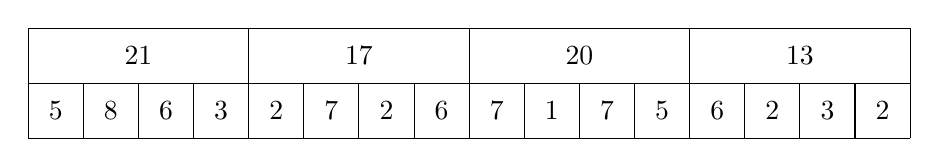
\begin{tikzpicture}[scale=0.7]
\draw (0,0) grid (16,1);

\draw (0,1) rectangle (4,2);
\draw (4,1) rectangle (8,2);
\draw (8,1) rectangle (12,2);
\draw (12,1) rectangle (16,2);

\node at (0.5, 0.5) {5};
\node at (1.5, 0.5) {8};
\node at (2.5, 0.5) {6};
\node at (3.5, 0.5) {3};
\node at (4.5, 0.5) {2};
\node at (5.5, 0.5) {7};
\node at (6.5, 0.5) {2};
\node at (7.5, 0.5) {6};
\node at (8.5, 0.5) {7};
\node at (9.5, 0.5) {1};
\node at (10.5, 0.5) {7};
\node at (11.5, 0.5) {5};
\node at (12.5, 0.5) {6};
\node at (13.5, 0.5) {2};
\node at (14.5, 0.5) {3};
\node at (15.5, 0.5) {2};

\node at (2, 1.5) {21};
\node at (6, 1.5) {17};
\node at (10, 1.5) {20};
\node at (14, 1.5) {13};

\end{tikzpicture}
\end{center}


En aquesta estructura, és fàcil modificar els elements del vector,
perquè només cal actualitzar la suma d'un sol bloc després de cada
modificació, i això es pot fer en temps $O(1)$. Per exemple, la imatge
següent mostra com canvia el valor d'un element i la suma del bloc
corresponent:


\begin{center}
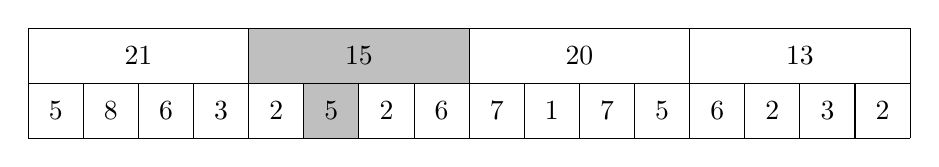
\begin{tikzpicture}[scale=0.7]
\fill[color=lightgray] (5,0) rectangle (6,1);
\draw (0,0) grid (16,1);

\fill[color=lightgray] (4,1) rectangle (8,2);
\draw (0,1) rectangle (4,2);
\draw (4,1) rectangle (8,2);
\draw (8,1) rectangle (12,2);
\draw (12,1) rectangle (16,2);

\node at (0.5, 0.5) {5};
\node at (1.5, 0.5) {8};
\node at (2.5, 0.5) {6};
\node at (3.5, 0.5) {3};
\node at (4.5, 0.5) {2};
\node at (5.5, 0.5) {5};
\node at (6.5, 0.5) {2};
\node at (7.5, 0.5) {6};
\node at (8.5, 0.5) {7};
\node at (9.5, 0.5) {1};
\node at (10.5, 0.5) {7};
\node at (11.5, 0.5) {5};
\node at (12.5, 0.5) {6};
\node at (13.5, 0.5) {2};
\node at (14.5, 0.5) {3};
\node at (15.5, 0.5) {2};

\node at (2, 1.5) {21};
\node at (6, 1.5) {15};
\node at (10, 1.5) {20};
\node at (14, 1.5) {13};

\end{tikzpicture}
\end{center}


Aleshores, per calcular la suma dels elements d'un rang, dividim el
rang en tres parts de manera que la suma consta de valors d'elements
individuals i sumes de blocs entre ells:


\begin{center}
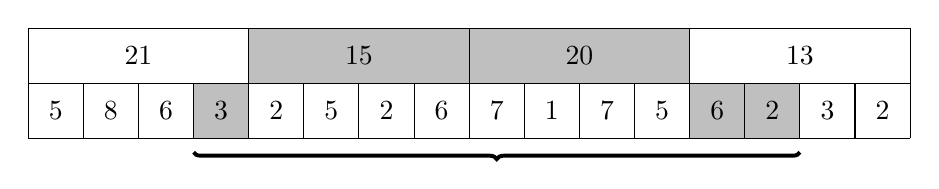
\begin{tikzpicture}[scale=0.7]
\fill[color=lightgray] (3,0) rectangle (4,1);
\fill[color=lightgray] (12,0) rectangle (13,1);
\fill[color=lightgray] (13,0) rectangle (14,1);
\draw (0,0) grid (16,1);

\fill[color=lightgray] (4,1) rectangle (8,2);
\fill[color=lightgray] (8,1) rectangle (12,2);
\draw (0,1) rectangle (4,2);
\draw (4,1) rectangle (8,2);
\draw (8,1) rectangle (12,2);
\draw (12,1) rectangle (16,2);

\node at (0.5, 0.5) {5};
\node at (1.5, 0.5) {8};
\node at (2.5, 0.5) {6};
\node at (3.5, 0.5) {3};
\node at (4.5, 0.5) {2};
\node at (5.5, 0.5) {5};
\node at (6.5, 0.5) {2};
\node at (7.5, 0.5) {6};
\node at (8.5, 0.5) {7};
\node at (9.5, 0.5) {1};
\node at (10.5, 0.5) {7};
\node at (11.5, 0.5) {5};
\node at (12.5, 0.5) {6};
\node at (13.5, 0.5) {2};
\node at (14.5, 0.5) {3};
\node at (15.5, 0.5) {2};

\node at (2, 1.5) {21};
\node at (6, 1.5) {15};
\node at (10, 1.5) {20};
\node at (14, 1.5) {13};

\draw [decoration={brace}, decorate, line width=0.5mm] (14,-0.25) -- (3,-0.25);

\end{tikzpicture}
\end{center}


Com que el nombre d'elements individuals és $O(\sqrt n)$ i el nombre
de blocs també és $O(\sqrt n)$, calcular la suma triga temps $O(\sqrt
n)$.  Per què triem $\sqrt n$ com a mida de bloc? Perquè és la mida
que \emph{equilibra} ambdues operacions: el vector es divideix en
$\sqrt n$ blocs, cadascun dels quals conté $\sqrt n$ elements.

A la pràctica, no és necessari triar el valor exacte de $\sqrt n$, i
en canvi podem fer servir $k$ i $n/k$ on $k$ és diferent de $\sqrt
n$. El paràmetre òptim depèn del problema i de l'entrada. Per exemple,
si un algorisme passa sovint pels blocs però rarament inspecciona
elements únics dins dels blocs, seria preferible triar $k < \sqrt n$
blocs, cadascun dels quals conté $n/k > \sqrt n$ elements.

\section{Combinació d'algorismes}

En aquesta secció discutim dos algorismes d'arrel quadrada que es
basen en combinar dos algorismes en un de sol. En ambdós casos,
podríem fer servir qualsevol dels algorismes sense l'altre i resoldre
el problema en temps $O(n^2)$. Tanmateix, combinant els algorismes, el
temps d'execució és només $O(n\sqrt n)$.

\subsubsection{Processament per casos}

Suposem que se'ns dóna una taula bidimensional que conté $n$
cel·les. Cada cel·la té una lletra assignada, i la nostra tasca és
trobar dues cel·les amb la mateixa lletra la distància de les quals
sigui mínima, on la distància entre les cel·les $(x_1,y_1)$ i
$(x_2,y_2)$ és $|x_1-x_2|+|y_1-y_2|$. Per exemple, considereu la
taula següent:


\begin{center}
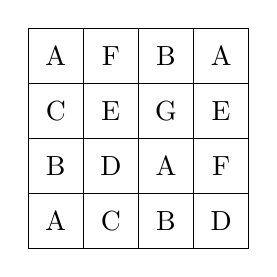
\begin{tikzpicture}[scale=0.7]
\node at (0.5,0.5) {A};
\node at (0.5,1.5) {B};
\node at (0.5,2.5) {C};
\node at (0.5,3.5) {A};
\node at (1.5,0.5) {C};
\node at (1.5,1.5) {D};
\node at (1.5,2.5) {E};
\node at (1.5,3.5) {F};
\node at (2.5,0.5) {B};
\node at (2.5,1.5) {A};
\node at (2.5,2.5) {G};
\node at (2.5,3.5) {B};
\node at (3.5,0.5) {D};
\node at (3.5,1.5) {F};
\node at (3.5,2.5) {E};
\node at (3.5,3.5) {A};
\draw (0,0) grid (4,4);
\end{tikzpicture}
\end{center}
En aquest cas, la distància mínima entre les dues lletres ``E'' és 2.

Podem resoldre el problema considerant cada lletra per separat. Amb
aquest enfocament, el nou problema és calcular la distància mínima
entre dues cel·les amb una lletra \emph{fixa} $c$. Ens centrem en dos
algorismes que resolen aquest problema:

\emph{Algorisme 1:} Recorre tots els parells de cel·les amb la lletra
$c$ i calcula la distància mínima entre aquestes cel·les. Això triga
$O(k^2)$, on $k$ és el nombre de cel·les amb la lletra $c$.

\emph{Algorisme 2:} Realitza una cerca d'amplada que comenci
simultàniament a cada cel·la amb la lletra $c$. Trobar la distància
mínima entre dues cel·les amb la lletra $c$ triga temps $O(n)$.

Una manera de resoldre el problema és escollir qualsevol dels
algorismes i utilitzar-lo per a totes les lletres. Si fem servir
l'algorisme 1, el temps d'execució és $O(n^2)$, perquè totes les
cel·les poden contenir la mateixa lletra, i en aquest cas $k=n$. A
més, si fem servir l'algorisme 2, el temps d'execució és $O(n^2)$,
perquè totes les cel·les poden tenir lletres diferents, i en aquest
cas necessitem $n$ cerques.

Tanmateix, podem \emph{combinar} els dos algorismes i utilitzar
algorismes diferents per a lletres diferents en funció de quantes
vegades apareix cada lletra a la taula. Suposem que una lletra $c$
apareix $k$ vegades. Si $k \le \sqrt n$, fem servir l'algorisme 1, i
si $k > \sqrt n$, fem servir l'algorisme 2. Veurem ara que si fem
això, el temps total d'execució de l'algorisme és només $O(n \sqrt
n)$.

Primer, suposem que fem servir l'algorisme 1 per a una lletra $c$. Com
que $c$ apareix com a màxim $\sqrt n$ vegades a la taula, comparem
cada cel·la amb la lletra $c$ com a molt $O(\sqrt n)$ vegades amb
altres cel·les. Així, el temps utilitzat per processar les com a molt
$n$ caselles amb lletres on es fa servir l'algorisme 1 és $O(n \sqrt
n)$. Ara, suposem que fem servir l'algorisme 2 per a una lletra
$c$. Hi ha com a màxim $\sqrt n$ d'aquestes lletres, de manera que
processar aquestes lletres també triga $O(n \sqrt n)$ temps.

\subsubsection{Processament per lots}

El nostre següent problema també tracta d'una taula bidimensional que
conté $n$ cel·les. Inicialment, cada cel·la excepte una és
blanca. Realitzem $n-1$ operacions, cadascuna de les quals calcula
primer la distància mínima des d'una cel·la blanca donada a una cel·la
negra, i després pinta la cel·la blanca de negre.

Per exemple, considereu l'operació següent:


\begin{center}
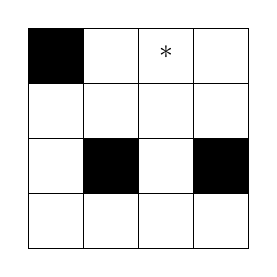
\begin{tikzpicture}[scale=0.7]
\fill[color=black] (1,1) rectangle (2,2);
\fill[color=black] (3,1) rectangle (4,2);
\fill[color=black] (0,3) rectangle (1,4);
\node at (2.5,3.5) {*};
\draw (0,0) grid (4,4);
\end{tikzpicture}
\end{center}


Primer, calculem la distància mínima des de la cel·la blanca marcada
amb * fins a una cel·la negra. La distància mínima és 2, perquè podem
moure dos passos a l'esquerra fins a una cel·la negra. Aleshores,
pintem la cèl·lula blanca de negre:


\begin{center}
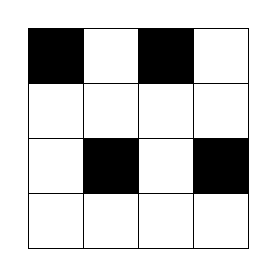
\begin{tikzpicture}[scale=0.7]
\fill[color=black] (1,1) rectangle (2,2);
\fill[color=black] (3,1) rectangle (4,2);
\fill[color=black] (0,3) rectangle (1,4);
\fill[color=black] (2,3) rectangle (3,4);
\draw (0,0) grid (4,4);
\end{tikzpicture}
\end{center}


Considereu els dos algorismes següents:

\emph{Algorisme 1:} Fem cerca en amplada per calcular per a cada
cel·la blanca la distància a la cel·la negra més propera. Això triga
temps $O(n)$, i després de la cerca, podem trobar la distància mínima
des de qualsevol cel·la blanca a una cel·la negra en temps $O(1)$.

\emph{Algorisme 2:} Mantenim una llista de cel·les pintades de
negre. Per a cada operació, recorrem la llista per trobar la cel·la
negra mes propera i, a continuació, afegim una nova cel·la a la
llista. Això triga $O(k)$ on $k$ és la longitud de la llista.

Podem combinar els algorismes anteriors dividint les operacions en
$O(\sqrt n)$ \emph{lots} (batches), cadascun dels quals consta de
$O(\sqrt n)$ operacions. Al començament de cada lot, fem servir
l'algorisme 1. A continuació, utilitzem l'algorisme 2 per processar
les operacions del lot. Netegem la llista de l'algorisme 2 entre els
lots. En cada operació, la distància mínima a una cel·la negra és la
distància calculada per l'algorisme 1 o la distància calculada per
l'algorisme 2.

L'algorisme resultant triga temps $O(n\sqrt n)$. Primer, l'algorisme 1
s'executa $O(\sqrt n)$ vegades, i cada cerca triga temps $O(n)$. En
segon lloc, quan s'utilitza l'algorisme 2 en un lot, la llista conté
$O(\sqrt n)$ cel·les (ja que netegem la llista entre els lots) i cada
operació triga temps $O(\sqrt n)$.

\section{Particions senceres}

Alguns algorismes d'arrel quadrada es basen en la següent observació:
si un nombre enter positiu $n$ es representa com a suma d'enters
positius, aquesta suma sempre conté com a màxim $O(\sqrt n)$ nombres
\emph{diferents}. La raó d'això és que per a construir una suma que
contingui un nombre màxim de nombres diferents, hauríem de triar
nombres \emph{petits}. Si triem els nombres $1,2,\ldots,k$, la suma
resultant és
\[\frac{k(k+1)}{2}.\]
Així, la quantitat màxima de nombres diferents és $k = O(\sqrt n)$. A
continuació mostrem dos problemes que es poden resoldre de manera
eficient amb aquesta observació.

\subsubsection{Motxilla}

Suposem que se'ns dóna una llista de pesos enters la suma dels quals
és $n$. La nostra tasca és esbrinar totes les sumes que es poden
formar mitjançant un subconjunt de pesos. Per exemple, si els pesos
són $\{1,3,3\}$, les sumes possibles són les següents:


\begin{itemize}[noitemsep]
\item $0$ (empty set)
\item $1$
\item $3$
\item $1+3=4$
\item $3+3=6$
\item $1+3+3=7$
\end{itemize}


Utilitzant l'enfocament estàndard de la motxilla (vegeu el
capítol~\ref{knapsack-problems}), el problema es pot resoldre de la
següent manera: definim una funció $\texttt{possible}(x,k)$ el valor
de la qual és 1 si la suma $x$ es pot formar mitjançant els primers $k$
pesos, i 0 en cas contrari. Com que la suma dels pesos és $n$, hi ha
com a màxim $n$ pesos i tots els valors de la funció es poden calcular
en temps $O(n^2)$ mitjançant la programació dinàmica.

Tanmateix, podem fer que l'algorisme sigui més eficient utilitzant el
fet que com a màxim hi ha $O(\sqrt n)$ pesos \emph{diferents}. Així,
podem processar els pesos en grups que consisteixen en pesos
similars. Podem processar cada grup en temps $O(n)$, i això produeix un
algorisme de temps $O(n \sqrt n)$.

La idea és utilitzar un vector que enregistri les sumes de pesos que
es poden formar utilitzant els grups processats fins ara. El vector
conté $n$ elements: l'element $k$ és 1 si es pot formar la suma $k$ i
0 en cas contrari. Per processar un grup de pesos, escanegem el vector
d'esquerra a dreta i registrem les noves sumes de pesos que es poden
formar utilitzant aquest grup i els grups anteriors\footnote{(N. del
T.)  Suposem que tenim un nou grup de $t$ pesos de pes $x$. Creem
un vector $v$ de $n$ elements, l'element $v[k]$ del qual és $m$ si es
pot formar la suma $k$ amb els pesos anteriors, $m$ pesos del
nou grup, i no és possible fer-ho amb $m-1$ pesos, i $v[k]=\infty$ si no
es pot formar la suma $k$ de cap manera.  En particular, $v[k] = 0$ si
$k$ es podia formar abans, i $v[k]=v[k-x]+1$ altrament. Amb aixó podem
omplir aquest vector d'esquerra a dreta en temps $O(n)$. Les sumes $k$ que
ens interessen són aquelles que compleixen $v[k]\le t$.}

\subsubsection{Construcció de cadenes}

Donada una cadena \texttt{s} de longitud $n$ i un conjunt de cadenes
$D$ la longitud total de les quals és $m$, considereu el problema de
comptar el nombre de maneres en què \texttt{s} es pot formar com una
concatenació de cadenes en $D$. Per exemple, si
$\texttt{s}=\texttt{ABAB}$ i
$D=\{\texttt{A},\texttt{B},\texttt{AB}\}$, hi ha 4 maneres:


\begin{itemize}[noitemsep]
\item $\texttt{A}+\texttt{B}+\texttt{A}+\texttt{B}$
\item $\texttt{AB}+\texttt{A}+\texttt{B}$
\item $\texttt{A}+\texttt{B}+\texttt{AB}$
\item $\texttt{AB}+\texttt{AB}$
\end{itemize}


Podem resoldre el problema mitjançant la programació dinàmica: Sigui
$\texttt{count}(k)$ el nombre de maneres de construir el
prefix $\texttt{s}[0 \ldots k]$ utilitzant les cadenes de $D$. Ara
$\texttt{count}(n-1)$ dóna la resposta al problema, i podem resoldre
el problema en $O(n^2)$ temps utilitzant una estructura trie.

No obstant això, podem resoldre el problema de manera més eficient
mitjançant l'ús d'un hash de cadenes i el fet que com a màxim hi ha
$O(\sqrt m)$ longituds de cadenes diferents a $D$. Primer, construïm
un conjunt $H$ que conté tots els valors hash de les cadenes de
$D$. Aleshores, quan calculem un valor de $\texttt{count}(k)$, passem
per tots els valors de $p$ de manera que hi hagi una cadena de
longitud $p$ a $D$, calculem el valor hash de
$\texttt{s}[k-p+1\ldots k]$ i comprovem si pertany a $H$. Com que hi ha
com a màxim $O(\sqrt m)$ longituds de cadena diferents, això resulta en un
algorisme de temps $O(n \sqrt m)$.

\section{Algorisme de Mo}

\index{Algorisme de Mo}

\key{Algorisme de Mo}\footnote{Segons \cite{cod15}, aquest algorisme
rep el nom de Mo Tao, un programador competitiu xinès, però la tècnica
ha aparegut anteriorment a la literatura \cite{ken06}.} es pot
utilitzar en molts problemes que requereixen processar consultes
d'interval en un vector \emph{estàtic}, és a dir, un vector amb valors que
no canvien entre consultes. En cada consulta, se'ns dóna un
rang $[a,b]$, i hauríem de calcular un valor basant-nos en els
elements del vector entre les posicions $a$ i $b$. Com que el vector
és estàtic, les consultes es poden processar en qualsevol ordre i
l'algorisme de Mo processa les consultes en un ordre especial que
garanteix que l'algorisme funciona de manera eficient.

L'algorisme de Mo manté un \emph{rang actiu} de la matriu, i la
resposta a una consulta sobre l'interval actiu es coneix en cada
moment. L'algorisme processa les consultes una per una i sempre mou
els punts finals de l'interval actiu inserint i eliminant elements. La
complexitat temporal de l'algorisme és $O(n \sqrt n f(n))$ on la matriu
conté $n$ elements, hi ha $n$ consultes i cada inserció i eliminació
d'un element triga temps $O(f(n))$.

El truc de l'algorisme de Mo és l'ordre en què es processen les
consultes: el matriu es divideix en blocs de $k=O(\sqrt n)$ elements i
una consulta $[a_1,b_1]$ es processa abans d'una consulta $ [a_2,b_2]$
si es compleix
\begin{itemize}
\item $\lfloor a_1/k \rfloor < \lfloor a_2/k \rfloor$ o
\item $\lfloor a_1/k \rfloor = \lfloor a_2/k \rfloor$ i $b_1 < b_2$.
\end{itemize}

Així, totes les consultes els extrems esquerres de les quals es troben
en un bloc determinat es processen una darrere l'altra ordenades
segons els seus extrems dret. Utilitzant aquest ordre, l'algorisme
només realitza $O(n \sqrt n)$ operacions, perquè el punt final
esquerre es mou $O(n)$ vegades $O(\sqrt n)$ passos, i el punt final
dret es mou $O(\sqrt n)$ vegades $O(n)$ passos. Així, ambdós extrems
mouen un total de $O(n \sqrt n)$ passos durant l'algorisme.

\subsubsection*{Exemple}

Com a exemple, considerem un problema on se'ns dóna un conjunt de
consultes, cadascuna d'elles corresponent a un interval del vector,
i la nostra tasca és calcular per a cada consulta el nombre d'elements
\emph{diferents} de l'interval.

En l'algorisme de Mo, les consultes sempre s'ordenen de la mateixa
manera, però segons el problema mantenim la resposta d'una manera o d'altra.
En aquest problema, mantenim un vector \texttt{count}
on $\texttt{count}[x]$ indica el nombre de vegades que apareix un
element $x$ a l'interval actiu.

Quan passem d'una consulta a una altra, l'interval actiu canvia. Per
exemple, si l'interval actual és
\begin{center}
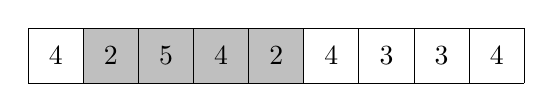
\begin{tikzpicture}[scale=0.7]
\fill[color=lightgray] (1,0) rectangle (5,1);
\draw (0,0) grid (9,1);
\node at (0.5, 0.5) {4};
\node at (1.5, 0.5) {2};
\node at (2.5, 0.5) {5};
\node at (3.5, 0.5) {4};
\node at (4.5, 0.5) {2};
\node at (5.5, 0.5) {4};
\node at (6.5, 0.5) {3};
\node at (7.5, 0.5) {3};
\node at (8.5, 0.5) {4};
\end{tikzpicture}
\end{center}
i el següent rang és
\begin{center}
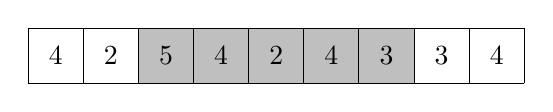
\begin{tikzpicture}[scale=0.7]
\fill[color=lightgray] (2,0) rectangle (7,1);
\draw (0,0) grid (9,1);
\node at (0.5, 0.5) {4};
\node at (1.5, 0.5) {2};
\node at (2.5, 0.5) {5};
\node at (3.5, 0.5) {4};
\node at (4.5, 0.5) {2};
\node at (5.5, 0.5) {4};
\node at (6.5, 0.5) {3};
\node at (7.5, 0.5) {3};
\node at (8.5, 0.5) {4};
\end{tikzpicture}
\end{center}
hi haurà tres passos: el punt final esquerre es mou un pas cap a la
dreta i el punt final dret es mou dos passos cap a la dreta.

Després de cada pas, el vector \texttt{count} s'ha
d'actualitzar. Després d'afegir un element $x$, augmentem el valor de
$\texttt{count}[x]$ en 1, i si $\texttt{count}[x]=1$ després d'això,
també augmentem la resposta a la consulta en 1. De la mateixa manera,
després d'eliminar un element $x$, disminuïm el valor de
$\texttt{count}[x]$ en 1, i si $\texttt{count}[x]=0$ després d'això,
també disminueix la resposta a la consulta en 1.

En aquest problema, el temps necessari per realitzar cada pas és
$O(1)$, de manera que l'algorisme triga temps $O(n \sqrt n)$.

